%%
%% Copyright (c) 2018-2019 Weitian LI <liweitianux@sjtu.edu.cn>
%% Creative Commons BY 4.0
%%

\chapter{射电晕对宇宙再电离探测的影响}
\label{chap:halo}

%=====================================================================
\section{评估方法}

利用上一章模拟得到的射电晕、EoR 信号以及其他前景成分的 SKA1-Low 观测图像,
于是可以定量地评估射电晕将对 EoR 探测产生的影响.
我们针对\ac{fgrm}和\ac{fgavd}两类前景处理方法 (\autoref{sec:fg-methods})
分别进行评估.
首先,我们计算一维\ac{ps}来对比射电晕和 EoR 信号在各个尺度 $k$ 的总体功率,
说明使用\ac{fgrm}方法时将面临的射电晕的污染强度.
其次,我们计算二维\ac{ps},然后在 EoR 窗口 (\autoref{sec:eor-window})
内比较射电晕和 EoR 信号的功率,
据此评估射电晕的污染将会对使用\ac{fgavd}方法产生多大程度的影响.

考虑一个有限宽的频带,信号(如前景辐射)将在频带的两端出现跃变,
这种边界效应会导致 Fourier 变换的结果具有显著的\ac{sidelobe}.
即使输入信号非常平滑,Fourier 变换后也会出现一系列幅度较大的高频 Fourier 成分,
如\autoref{fig:ft-sidelobes} 所示.
为了抑制边界效应所产生的\ac{sidelobe},可以先对信号加窗,然后再进行 Fourier 变换.
一个常用的选择是 Blackman--Nuttall \ac{winfunc},
该\ac{winfunc}具有良好的\ac{sidelobe}性质 \cite{nuttall1981}:
\begin{equation}
  w[n] = a_0 - a_1 \cos\left(\frac{2\Cpi n}{N}\right)
    + a_2 \cos\left(\frac{4\Cpi n}{N}\right)
    - a_3 \cos\left(\frac{6\Cpi n}{N}\right) ,
\end{equation}
其中
$N$ 为采样点的数目(即窗的宽度),
其他系数分别为:
$a_0 = 0.3635819$、
$a_1 = 0.4891775$、
$a_2 = 0.1365995$ 和
$a_3 = 0.0106411$.
\autoref{fig:ft-sidelobes} 显示了使用 Blackman--Nuttall \ac{winfunc}
之后得到的 Fourier 变换结果,可见高频 Fourier 成分的幅度被有效地抑制了.
因此,我们对上一章模拟得到的\ac{imgcube}沿频率方向施加
Blackman--Nuttall \ac{winfunc}然后再计算\ac{ps}
\cite{trott2015,chapman2016}.

\begin{figure}[htp]
  \centering
  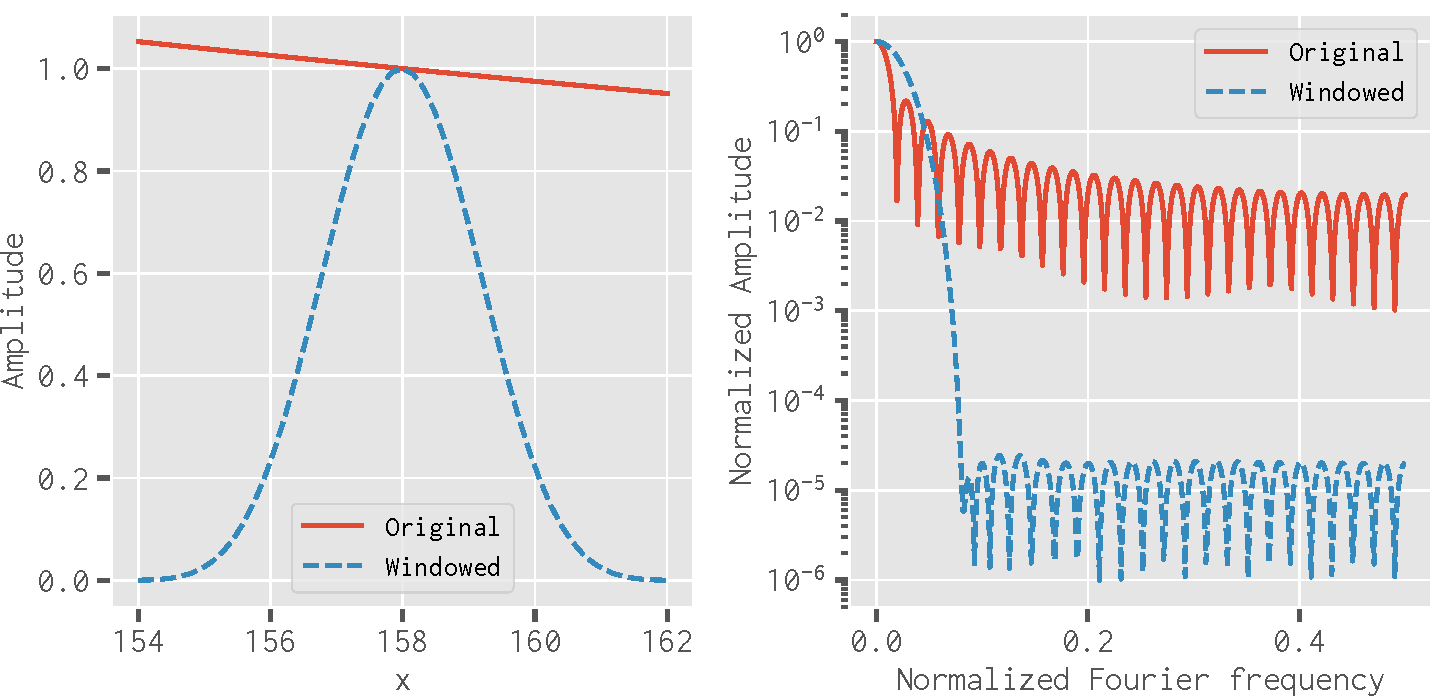
\includegraphics[width=\textwidth]{ft-sidelobes}
  \bicaption[加窗前后的 Fourier 变换结果对比]{%
    直接进行 Fourier 变换(红色实线)与
    使用 Blackman--Nuttall \acs*{winfunc}之后再 Fourier 变换(蓝色虚线)
    的结果对比.
    左栏显示了加窗前后的输入信号 $y = x^{-2}$,右栏显示了相应的 Fourier 变换结果.
  }{%
    A comparison of the Fourier transform results with and without
    applying the Blackman--Nuttall window function.
    The left panel shows the original input signal $y = x^{-2}$
    (solid red line) and the windowed signal (dashed blue line);
    the right panel shows the corresponding Fourier transform results.
  }
  \label{fig:ft-sidelobes}
\end{figure}


%=====================================================================
\section{一维功率谱}
\label{sec:ps1d}

\begin{figure}[htp]
  \centering
  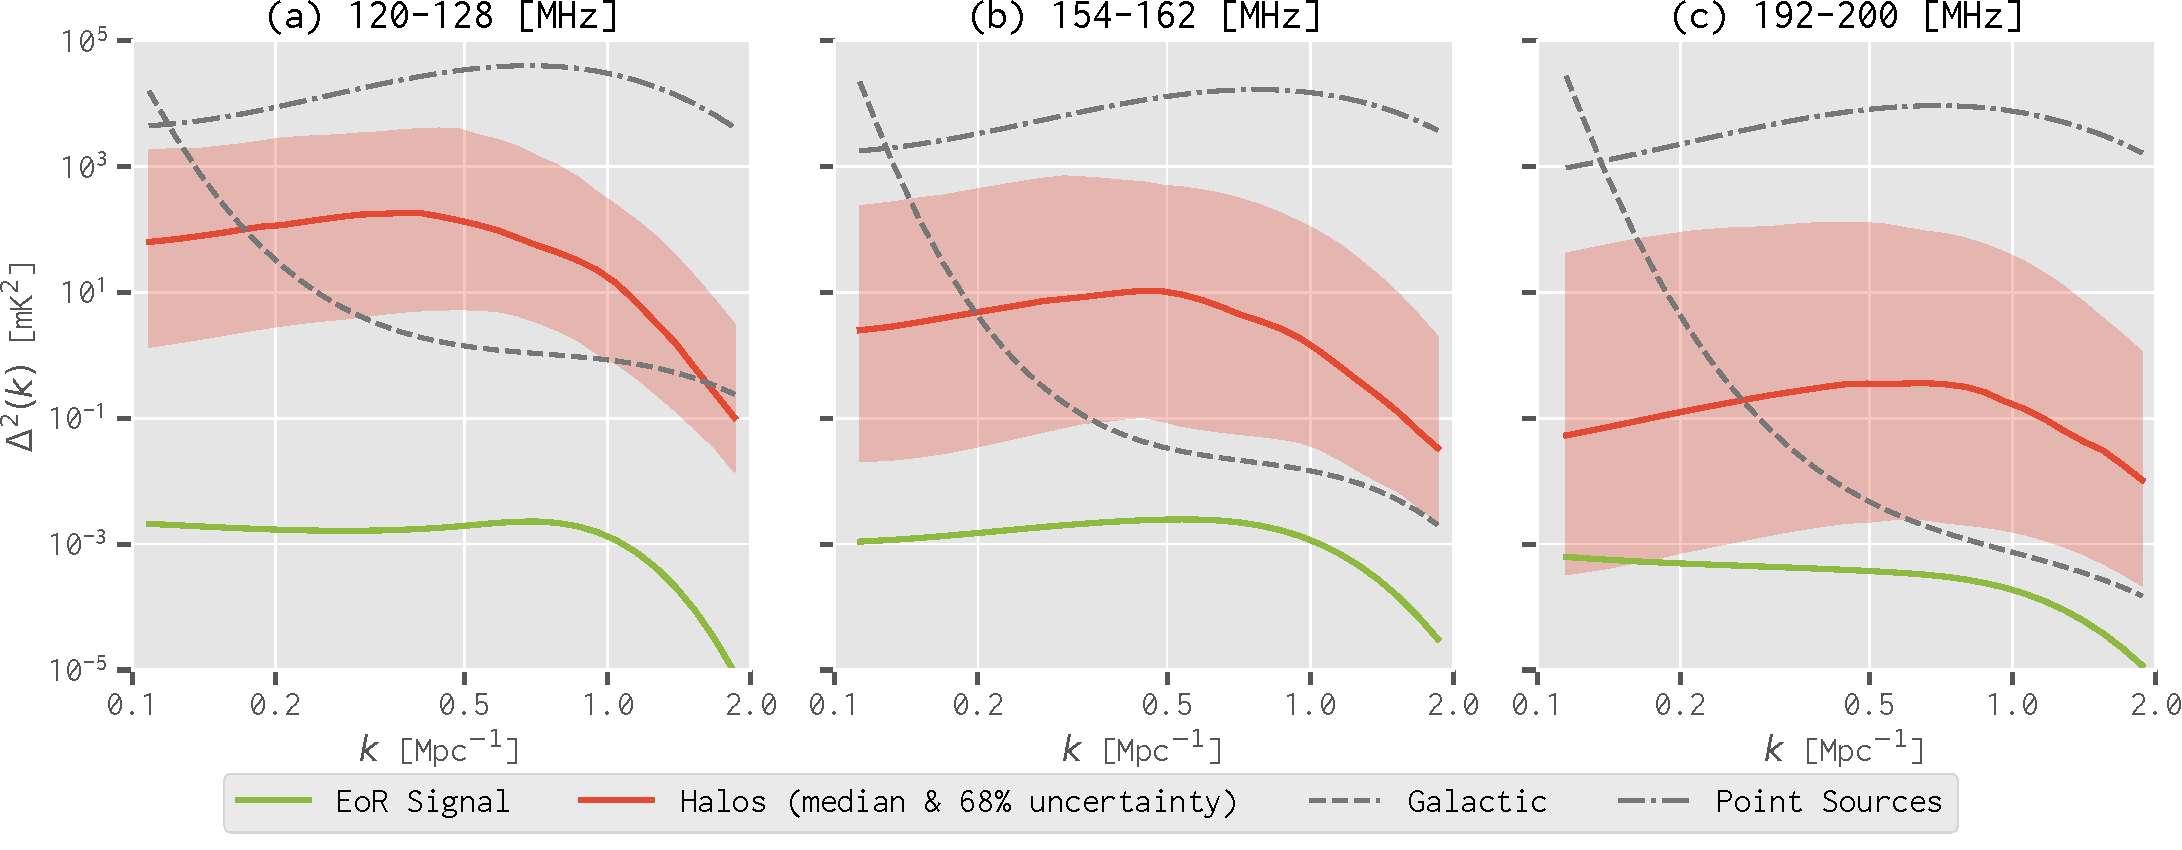
\includegraphics[width=\textwidth]{ps1d-3bands}
  \bicaption[各成分在三个频带内的一维功率谱 $\Delta^2(k)$ 对比]{%
    TODO...
  }{%
    Comparisons of the 1D dimensionless power spectra $\Delta^2(k)$
    among the EoR signal (solid green line), radio halos (solid red line),
    Galactic diffuse emission (dashed gray line), and extragalactic point
    sources (dash-dotted gray line) in the
    \textbf{(a)} \SIrange{120}{128}{\MHz},
    \textbf{(b)} \SIrange{154}{162}{\MHz}, and
    \textbf{(c)} \SIrange{192}{200}{\MHz} frequency bands.
    The solid red lines and shaded regions represent the median values
    and the corresponding 68\% uncertainties of the power
    spectra for radio halos estimated from the 100 simulation runs.
  }
  \label{fig:ps1d-3bands}
\end{figure}

We calculate the 1D dimensionless power spectra $\Delta^2(k)$ for each
image cube obtained in \autoref{sec:obs-simu}.
For radio halos, we make use of all the 100 simulation runs
(\autoref{sec:radio-halos}) to estimate the median power spectra and
the corresponding 68\% uncertainties.
The comparisons of the power spectra $\Delta^2(k)$ between radio halos
and the EoR signal in each frequency band are displayed
in \autoref{fig:ps1d-3bands}, where we also show the power spectra of
Galactic diffuse emission and extragalactic point sources for comparison.
The median power spectra (solid red lines) show that radio halos are
generally more luminous than the EoR signal by about
\numlist{e4; e3; e2.5} times
on scales of $\SI{0.1}{\per\Mpc} < k < \SI{2}{\per\Mpc}$
in the \numrange{120}{128}, \numrange{154}{162}, and \numrange{192}{200}
\si{\MHz} bands, respectively.
Given the large uncertainties in, e.g., brightness and number density,
of radio halos, the power spectra can vary by about \numrange{10}{100}
times with respect to the median values within the 68\%
uncertainties (red shaded regions).
We also find that, although on large scales
($k \lesssim \SI{0.1}{\per\Mpc}$) the Galactic foreground is the
strongest contaminating source, its power deceases rapidly as the
scale becomes smaller and is weaker than the median power of radio halos
by a factor of about \numrange{10}{100} on scales of
$\SI{0.5}{\per\Mpc} \lesssim k \lesssim \SI{1}{\per\Mpc}$
in all the three bands.
These results evidently show that radio halos are severe foreground
contaminating sources.
Moreover, it can be a major challenge to accurately model and remove radio
halos due to their diffuse and relatively complicated morphologies.


%=====================================================================
\section{二维功率谱}
\label{sec:ps2d}

\begin{figure}[htp]
  \centering
  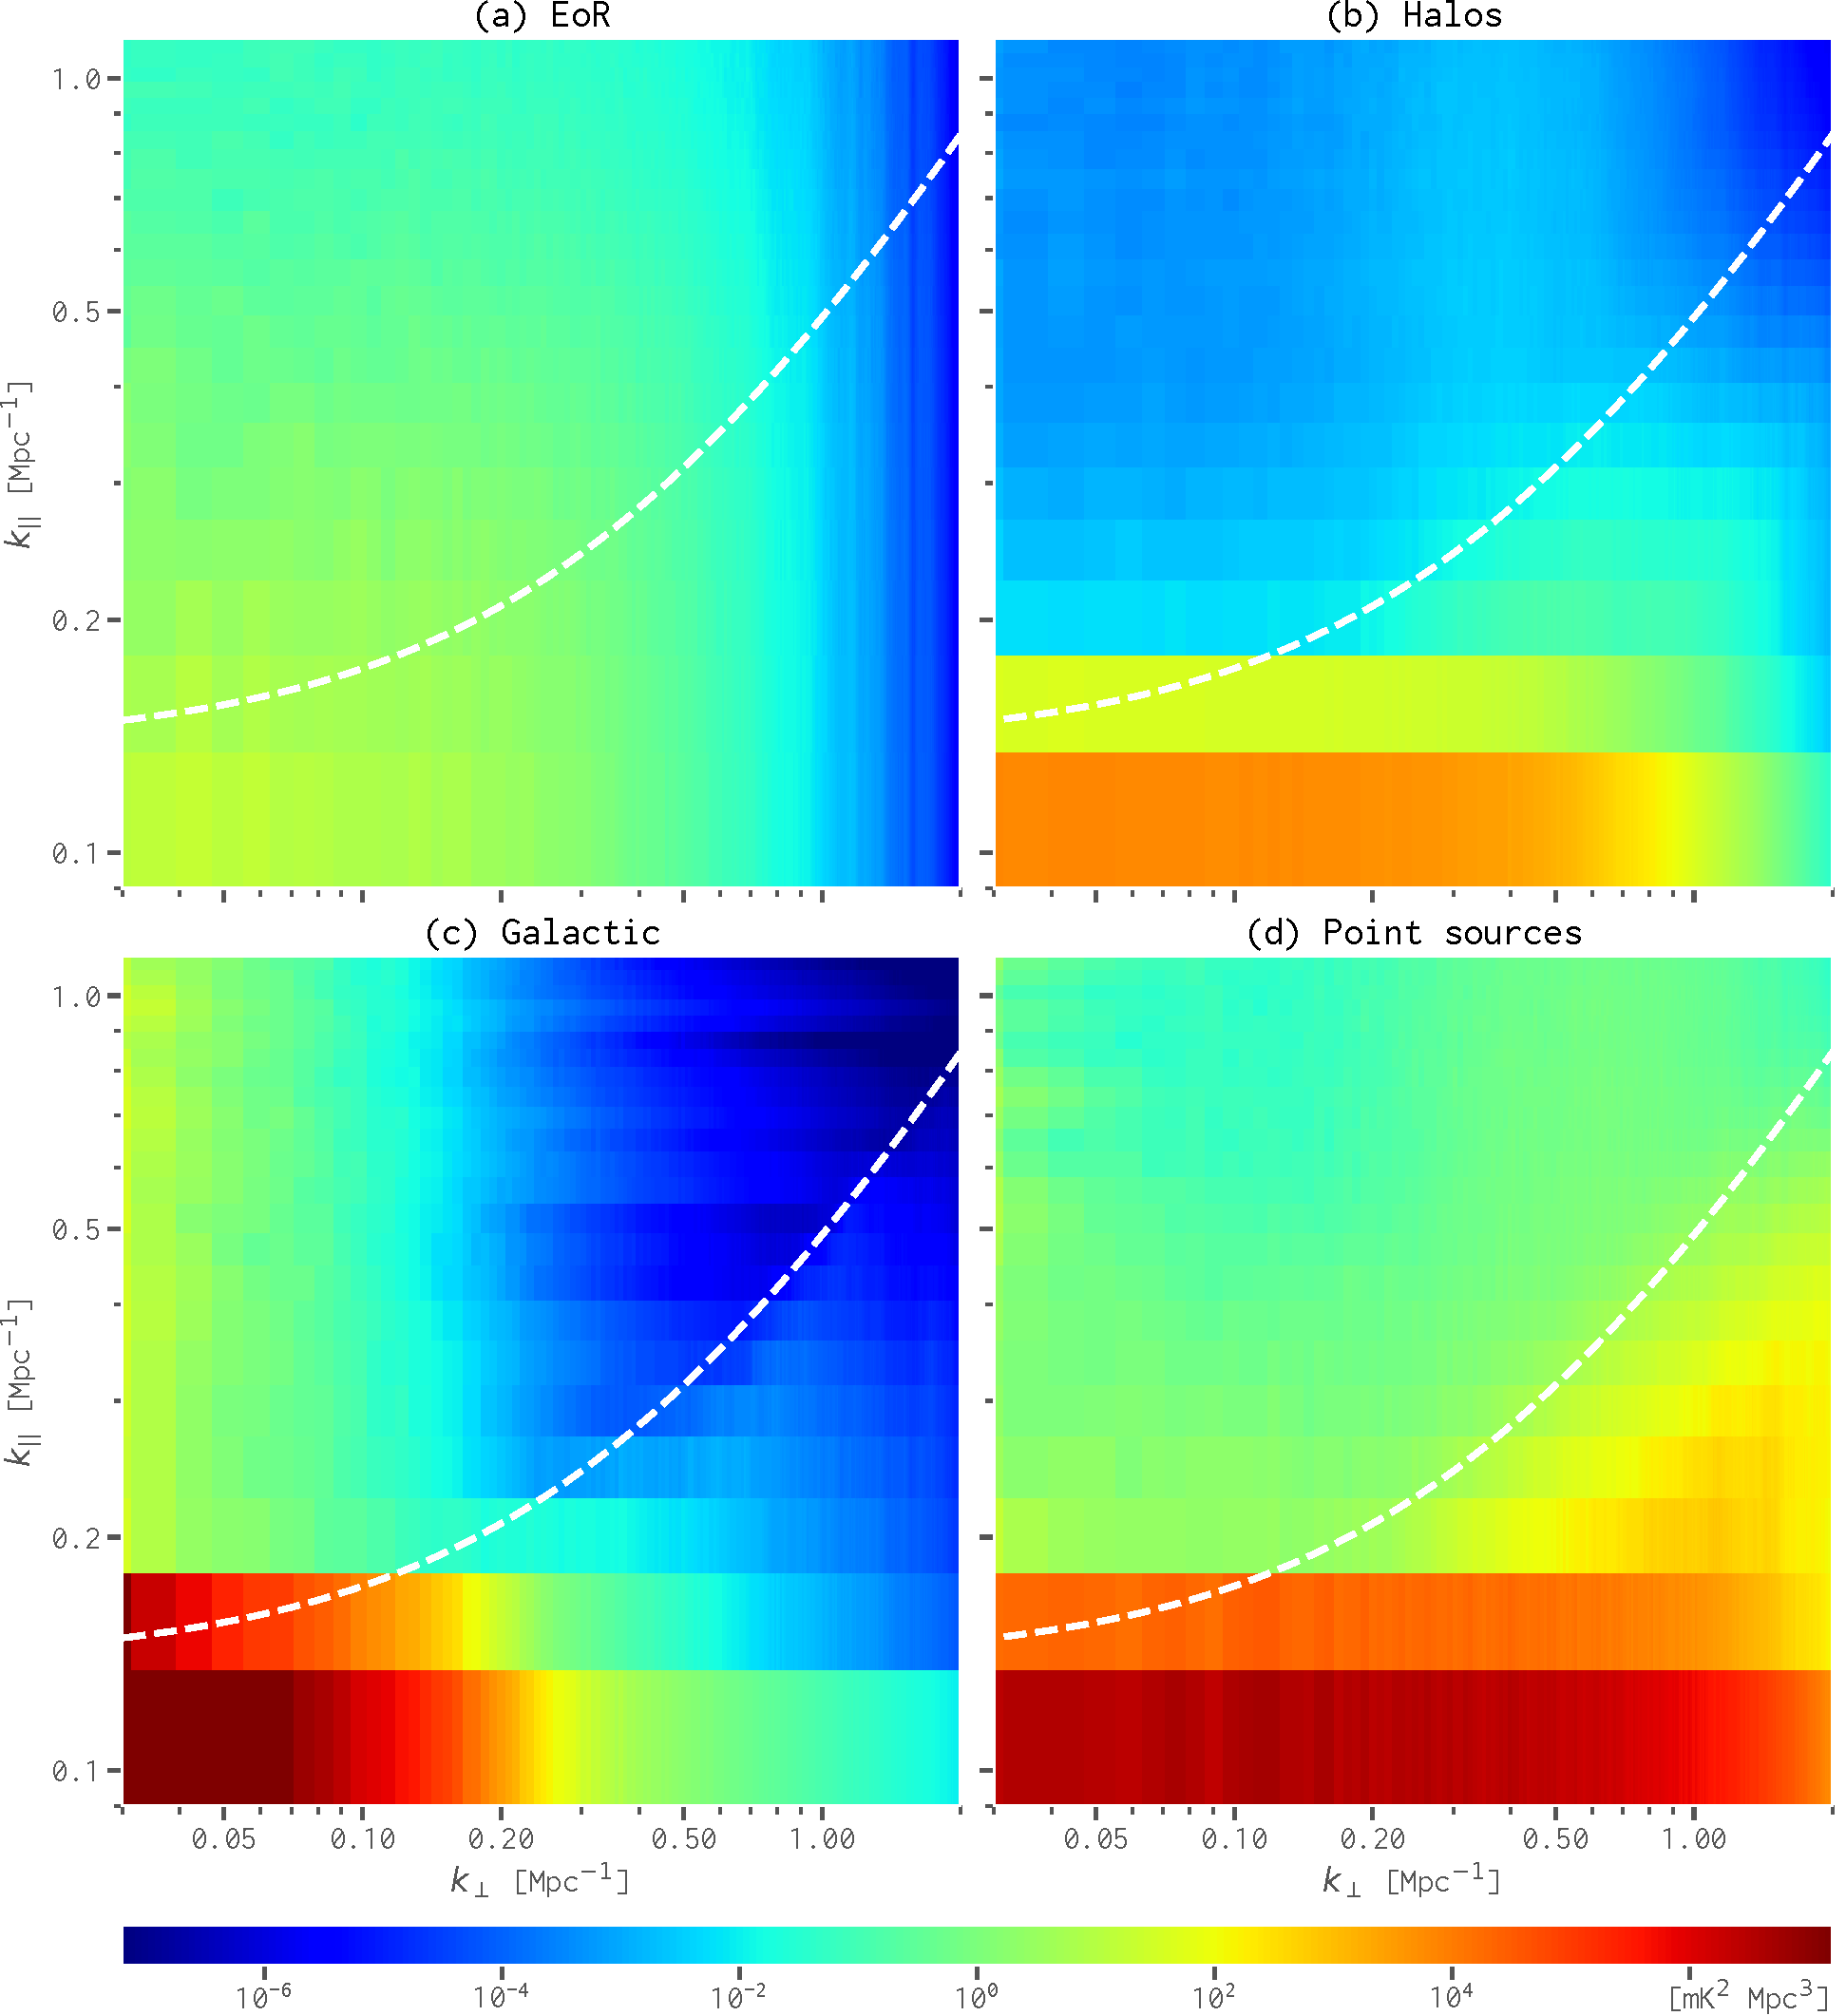
\includegraphics[width=\textwidth]{ps2d-band158}
  \bicaption[各成分在 \SIrange{154}{162}{\MHz} 频段的二维功率谱 $P(\kperp, \klos)$]{%
    TODO...
  }{%
    The \SIrange{154}{162}{\MHz} 2D power spectra $P(\kperp, \klos)$ of
    \textbf{(a)} the EoR signal,
    \textbf{(b)} radio halos (median of the 100 simulation runs),
    \textbf{(c)} Galactic diffuse emission,
    and
    \textbf{(d)} extragalactic point sources.
    All panels share the same logarithmic scale in units of
    [\si{\mK\squared\Mpc\cubed}].
    The dashed white lines mark the boundary between the EoR window
    (at the top left) and the contaminating wedge (at the bottom right).
  }
  \label{fig:ps2d}
\end{figure}

We take the \SIrange{154}{162}{\MHz} band as an example and show in
\autoref{fig:ps2d} the 2D power spectra $P(\kperp, \klos)$ of the EoR
signal, radio halos (the median power spectrum of the 100 simulation runs),
Galactic diffuse emission, and extragalactic point sources.
We find that, as shown in many previous works,
the EoR signal distributes its power across all \klos{} modes,
illustrating its rapid fluctuations along the line-of-sight dimension,
while the spectral-smooth foreground components dominate only in the
low-\klos{} regions ($\klos{} \lesssim \SI{0.2}{\per\Mpc}$).
With regard to the angular dimension, the power of radio halos appears in
the range of $\kperp \lesssim \SI{1}{\per\Mpc}$, showing a concentration
on the intermediate scales of $\kperp \sim \SI{0.5}{\per\Mpc}$.
Meanwhile, the powers of Galactic diffuse emission and extragalactic
point sources dominate on the large scales of
$\kperp \lesssim \SI{0.1}{\per\Mpc}$ and a broad angular scales of
$\kperp \gtrsim \SI{0.1}{\per\Mpc}$, respectively.
These results are also consistent with \autoref{fig:ps1d-3bands}(b).

\begin{figure}[htp]
  \centering
  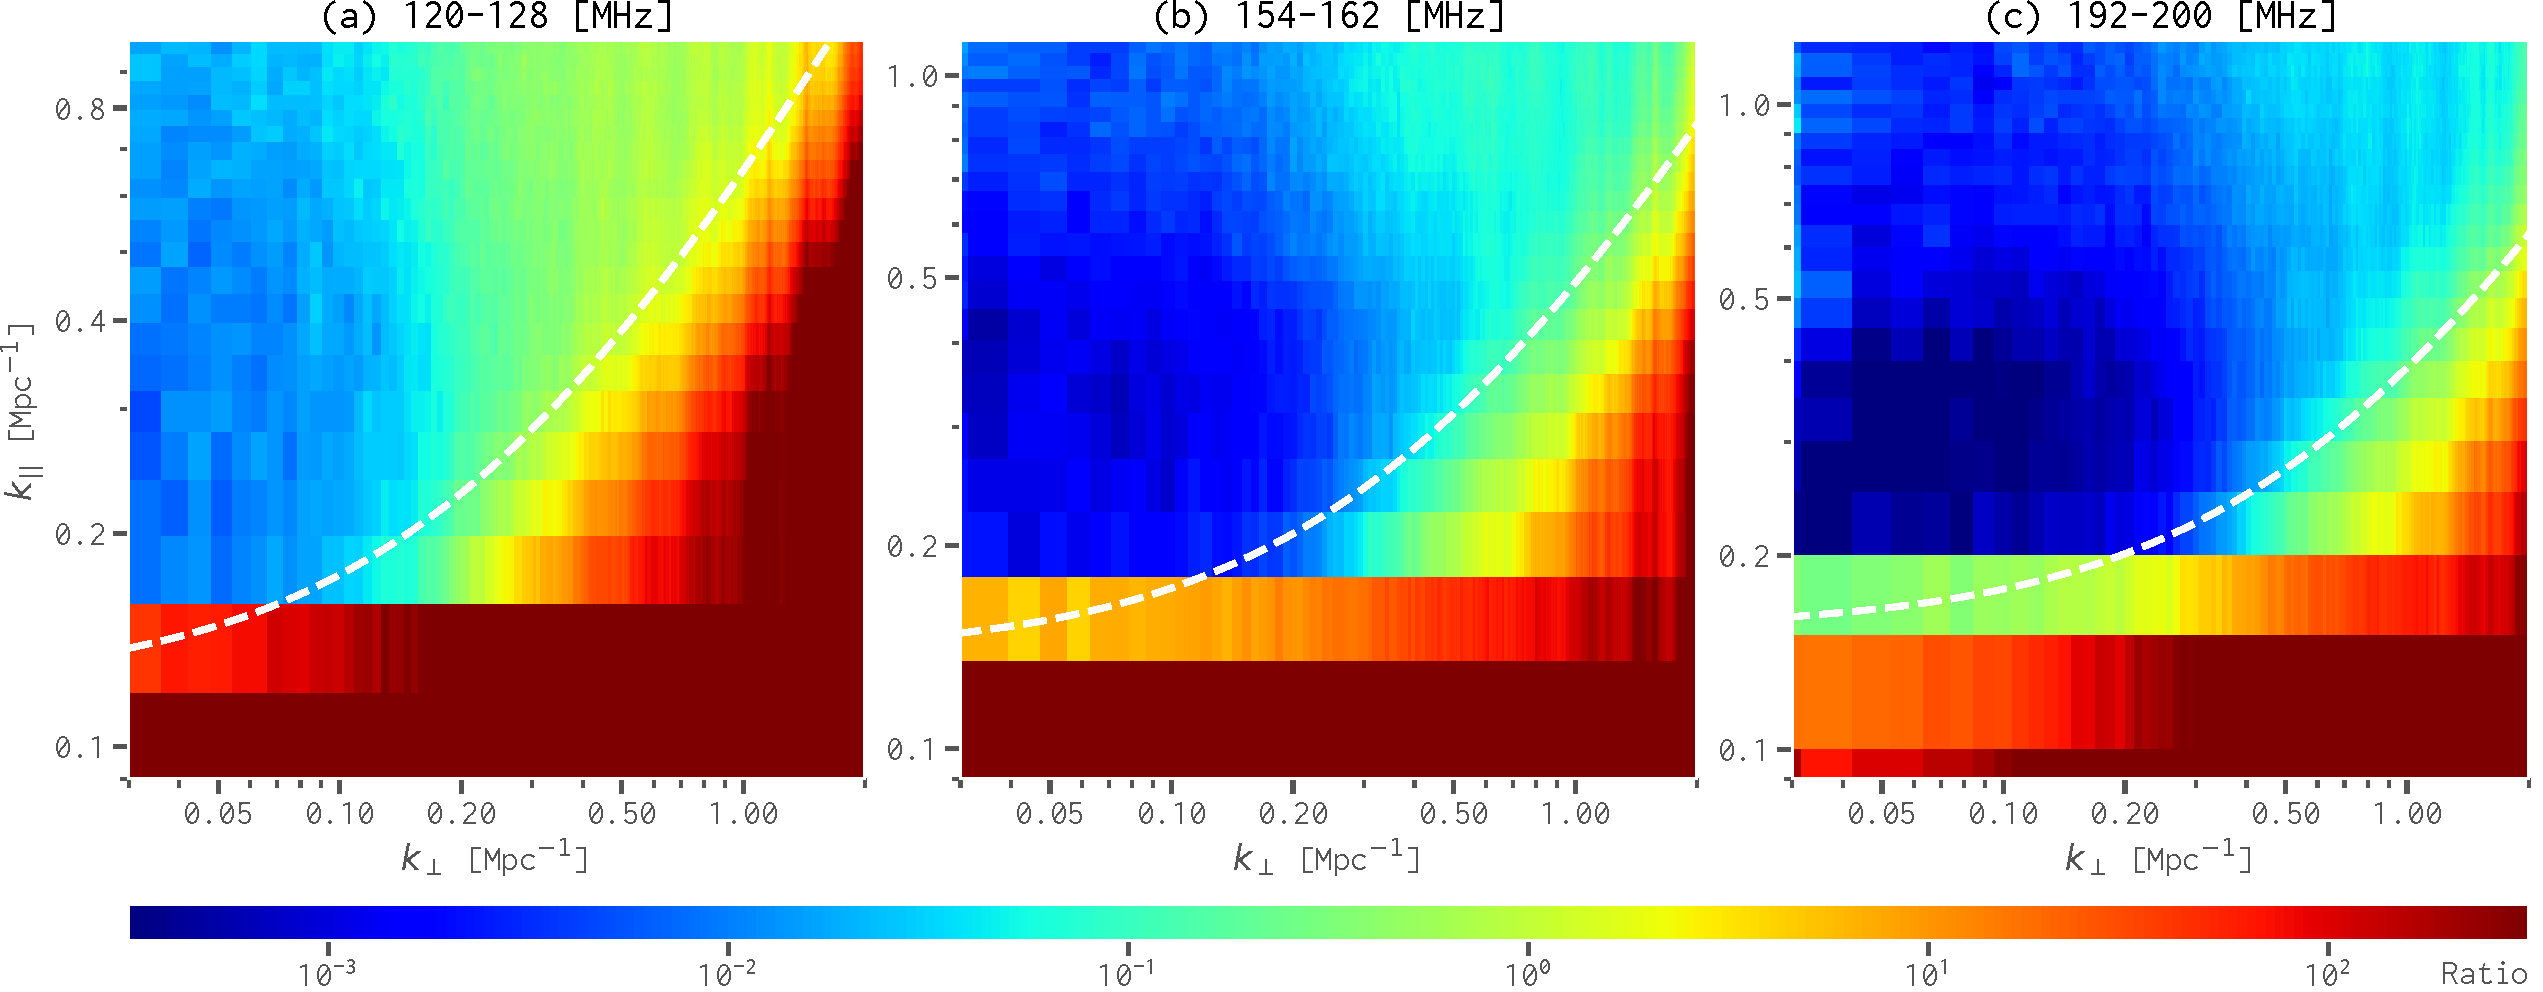
\includegraphics[width=\textwidth]{ps2d-ratio-3bands}
  \bicaption[射电晕和 EoR 信号的二维功率比 $R(\kperp, \klos)$]{%
    TODO...
  }{%
    The 2D power spectrum ratios $R(\kperp, \klos)$ of radio halos to the
    EoR signal in the
    \textbf{(a)} \SIrange{120}{128}{\MHz},
    \textbf{(b)} \SIrange{154}{162}{\MHz}, and
    \textbf{(c)} \SIrange{192}{200}{\MHz} frequency bands.
    The median 2D power spectrum of 100 simulation runs for radio halos
    is used.
    All panels use the same color bar in logarithmic scale.
    The dashed white lines mark the EoR window boundaries.
  }
  \label{fig:ps2d-ratio}
\end{figure}

In order to better evaluate the importance of radio halos as foreground
contaminating sources, we calculate the 2D power spectrum ratios
$R(\kperp, \klos)$ that are obtained by dividing the median 2D power
spectra of radio halos by those of the EoR signal in each frequency band.
We find that, as shown in \autoref{fig:ps2d-ratio}, the EoR measurements
will be significantly affected by radio halos on angular scales of
$\gtrsim \SI{0.1}{\per\Mpc}$, $\gtrsim \SI{0.3}{\per\Mpc}$, and
$\gtrsim \SI{0.5}{\per\Mpc}$ in the \numrange{120}{128},
\numrange{154}{162}, and \numrange{192}{200} \si{\MHz} bands, respectively.
It is also clearly shown that radio halos turn to cause stronger
contamination at lower frequencies (\SI{\sim 120}{\MHz}) than at higher
frequencies (\SI{\sim 200}{\MHz}).

\begin{figure}[htp]
  \centering
  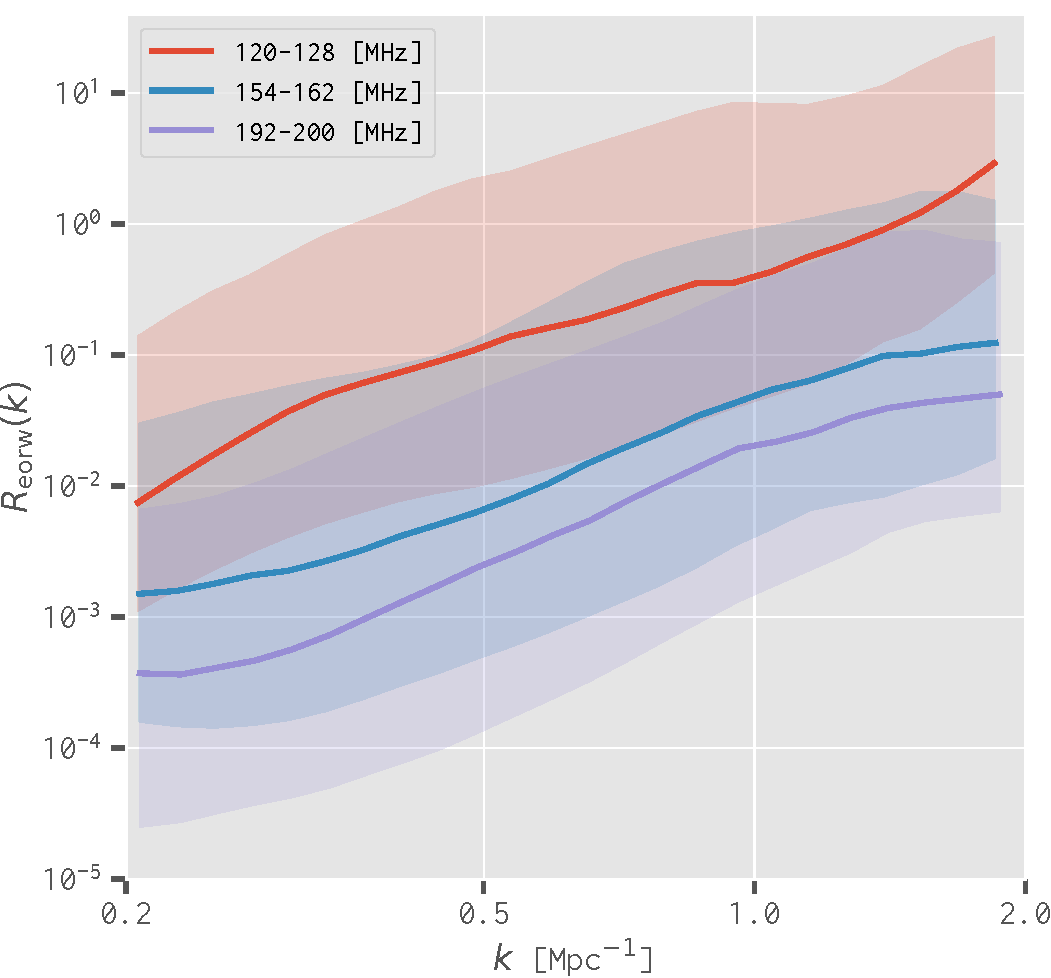
\includegraphics[width=0.8\textwidth]{ps1d-ratio-3bands}
  \bicaption[射电晕和 EoR 信号在 EoR 窗口内的一维功率比 $R_{\R{eorw}}(k)$]{%
    TODO...
  }{%
    The 1D power ratios $R_{\R{eorw}}(k)$ inside the EoR window of
    radio halos to the EoR signal.
    The solid lines and shaded regions show the median values and
    corresponding 68\% uncertainties, respectively.
  }
  \label{fig:ps1d-ratio}
\end{figure}

To further quantify the contamination caused by radio halos when
foreground avoidance methods are applied, we need to appropriately
define an EoR window in the $(\kperp, \klos)$ plane to avoid the
heavily contaminated areas and then compare the powers of radio halos
and the EoR signal derived inside the window.
We have tested multiple parameter configurations ($w$, $\Theta$) as
defined in \autoref{eq:eor-window}, and find that when $w = 3$ and
$\Theta$ being about 1.5 times the SKA1-Low's FoV (i.e.,
$\Theta = \SI{7.5}{\degree}$, \SI{6.0}{\degree}, and \SI{4.8}{\degree}
in \numrange{120}{128}, \numrange{154}{162}, and \numrange{192}{200}
\si{\MHz} bands, respectively) are used, a conservative EoR window
boundary can be defined to well avoid the contaminating wedge
(Figures~\ref{fig:ps2d} and \ref{fig:ps2d-ratio}).
However, a significant part (about 55\%, 54\%, and 40\% in
\numrange{120}{128}, \numrange{154}{162},
and \numrange{192}{200} \si{\MHz} bands, respectively) of the power of
the EoR signal is lost in the excised wedges.
By averaging the modes only inside the defined EoR window, we calculate
the 1D power spectrum ratios $R_{\R{eorw}}(k)$ of radio halos to the EoR
signal and present the results in \autoref{fig:ps1d-ratio}.
We find that, compared to \autoref{fig:ps1d-3bands}, the 1D power ratios
inside the EoR window $R_{\R{eorw}}(k)$ are suppressed by about 4 orders
of magnitude, which demonstrates that the EoR window is a powerful tool
in detecting the EoR signal.
For example, $R_{\R{eorw}}(k)$ on scales of $k \sim \SI{1}{\per\Mpc}$ are
generally about 45\%, 6\%, and 2\% in the \numrange{120}{128},
\numrange{154}{162}, and \numrange{192}{200} \si{\MHz} bands, respectively.
However, the power of radio halos leaked into the EoR window can still be
significant, considering that $R_{\R{eorw}}(k)$ on scales of
$\SI{0.5}{\per\Mpc} \lesssim k \lesssim \SI{1}{\per\Mpc}$ can be up to
about \numrange{230}{800}\%, \numrange{18}{95}\%, and
\numrange{7}{40}\% in the three frequency bands within the
68\% uncertainties (shaded regions).

Based on the above results, we conclude that radio halos are severe
foreground contaminating sources to EoR observations.
Even if inside the EoR window where most of the strong foreground
contamination is avoided, radio halos can still imprint
non-negligible contamination on the EoR measurements, especially at
lower frequencies (\SI{\sim 120}{\MHz}).
Careful treatments of radio halos as well as other foreground contaminating
sources would be indispensable for obtaining an EoR window that is not only
sufficiently clean but also as large as possible to preseve maximum
information of the EoR signal.


%=====================================================================
\section{伪频谱结构的影响}
\label{sec:freq-artifacts}

In practical observations with low-frequency radio interferometers, the
situations are much more complicated than our simulations.
For example, calibration uncertainties (e.g., insufficient sky modeling)
as well as other complicated instrumental and observational effects
(e.g., cable signal reflections, ionospheric distortions) can cause
frequency artifacts in the derived image cubes.

The smoothness along the frequency dimension is the most crucial feature
of various foreground components and is the key to extract the faint EoR
signal.
However, frequency artifacts may present in the obtained image cubes due
to calibration uncertainties and various instrumental and observational
effects, which break the spectral smoothness of the foreground emission
and hence damage the EoR measurements.

To evaluate the influence of the frequency artifacts on the power
spectra, we multiply each slice of the image cube by a random number
drawn from a Gaussian distribution with unity mean and then compare
the resulting power spectra \cite{chapman2016}.
Some simulation and observation studies have suggested that the residual
calibration errors in frequency channels may be about \numrange{0.1}{1}\%
\cite{barry2016,beardsley2016,ewallWice2017}.
We thus investigate two extreme cases here:
a frequency artifact of amplitude $A_{\R{arti}} = 0.1\%$ by
using $\sigma = 0.001$ for the Gaussian distribution,
and a frequency artifact of $A_{\R{arti}} = 1\%$ with $\sigma = 0.01$.

\begin{figure}[htp]
  \centering
  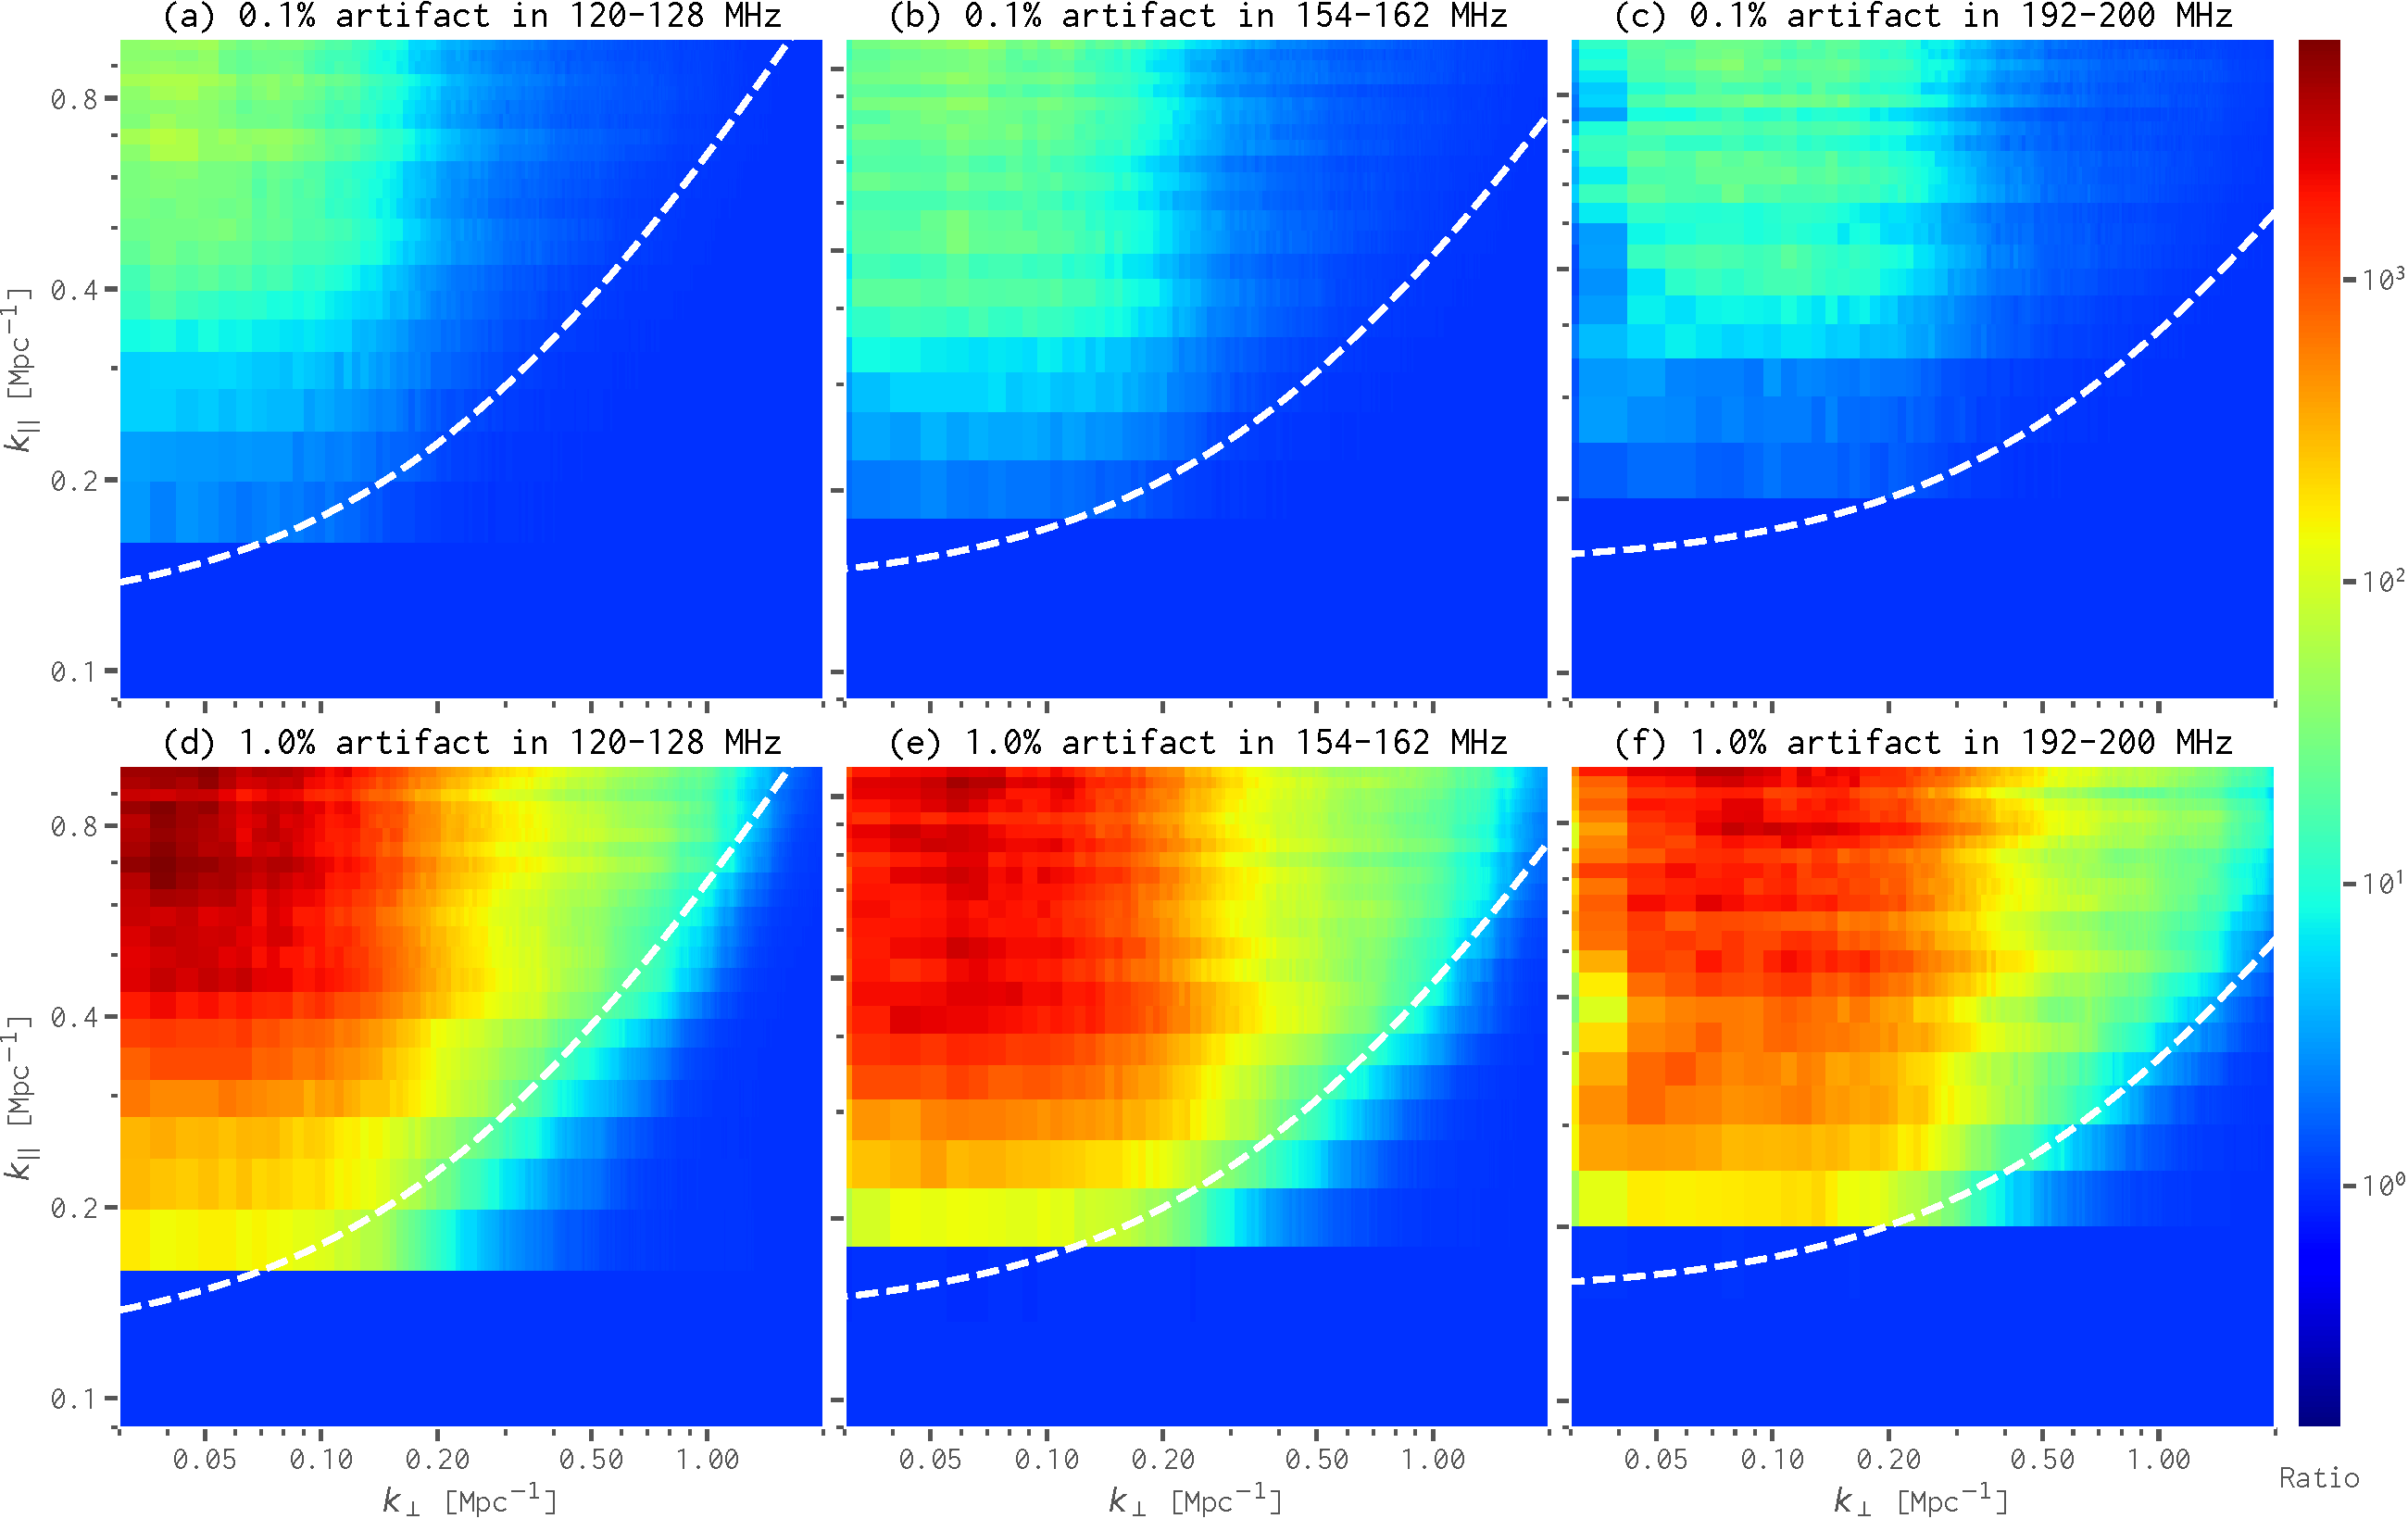
\includegraphics[width=\textwidth]{ps2d-ratio-crp-3bands}
  \bicaption[有无频谱伪结构时射电晕的二维功率比 $R_{\R{arti}}(\kperp, \klos)$]{%
    TODO...
  }{%
    The 2D power spectrum ratios $R_{\R{arti}}(\kperp, \klos)$ of radio
    halos that are obtained between the modified image cubes with
    frequency artifacts and the original ones.
    All the 100 simulation runs for radio halos are used to derive
    the median 2D power spectrum ratios that are presented here.
    The upper and lower rows show the cases of frequency artifacts
    being $A_{\R{arti}} = 0.1\%$ and $A_{\R{arti}} = 1\%$, respectively.
    The left, middle, and right columns show the power spectrum ratios
    in the \numrange{120}{128}, \numrange{154}{162}, and
    \numrange{192}{200} \si{\MHz} bands, respectively.
    The dashed white lines mark the EoR window boundaries.
    All panels share the same color bar in logarithmic scale.
  }
  \label{fig:ps2d-ratio-crp}
\end{figure}

For each of the 100 simulation runs for radio halos, we calculate the
2D power spectrum ratios $R_{\R{arti}}(\kperp, \klos)$ of the modified
image cube with the frequency artifact to the original one
(\autoref{sec:obs-simu}),
and present the median 2D power spectrum ratios obtained in the
\numrange{120}{128}, \numrange{154}{162}, and \numrange{192}{200}
\si{\MHz} bands with either $A_{\R{arti}} = 0.1\%$ or 1\% in
\autoref{fig:ps2d-ratio-crp}.
We find that, when the frequency artifact is added, the resulting 2D
power spectra are seriously damaged in all three frequency bands.
On scales of $\kperp \lesssim \SI{0.2}{\per\Mpc}$ and
$\klos \gtrsim \SI{0.3}{\per\Mpc}$,
adding frequency artifact of $A_{\R{arti}} = 0.1\%$
causes the power of radio halos to be about 17, 15, and 13 times
stronger in the \numrange{120}{128},
\numrange{154}{162}, and \numrange{192}{200} \si{\MHz} bands,
respectively, and the corresponding power increases are about
1700, 1500, and 1300 times
for frequency artifact of $A_{\R{arti}} = 1\%$.
As a comparison, we add the same frequency artifacts
($A_{\R{arti}} = 0.1\%$ and 1\%) to the image
cubes of the EoR signal, but find that the changes in the calculated
2D power spectra are negligible.
This is because the EoR signal already fluctuates remarkably along
the frequency dimension.
Consequently, even very minor (\num{\sim 0.1}\%) instrumental or
calibration errors can make the contamination of radio halos
become much stronger, particularly inside the critical EoR window.
These results further support our conclusion made in \autoref{sec:ps2d}
that radio halos are important foreground sources and must be carefully
dealt with in EoR experiments.


%=====================================================================
\section{远旁瓣的影响}
\label{sec:fscn}

Phased arrays, which are widely used in low-frequency radio
interferometers (e.g., LOFAR, MWA, SKA1-Low), usually have complicated
beam profiles.
Sources far from the main lobe of the station beam can introduce
noise-like corruptions, known as the far side-lobe confusion noise
(FSCN; \citeay{smirnov2012}), to images through the multitude of
side-lobes.
FSCN will not decrease once the $uv$ coverage of the observation no
longer improves, and can be the limiting factor in the noise
performance of interferometers \cite{mort2017}.

To investigate the impacts of FSCN contributed by the radio halos
located in the far side-lobes of the station beam, we have generated
the corresponding sky model for the \texttt{OSKAR} simulator,
which evaluates the radio interferometer measurement equation
\cite{smirnov2011} and is able to perform full-sky simulations with
realistic beam profiles.
More details about the beam shapes and side-lobe properties of the
SKA1-Low can be found in \citeay{mort2017}.
As an example, we simulate the radio halos in the \SIrange{154}{162}{\MHz}
band that cover the sky from the edge of the second side-lobe
($\phi \sim \SI{10}{\degree}$ from the field center) to the horizon
($\phi = \SI{90}{\degree}$).
This emulates an ideal CLEAN procedure in practical data analysis that
removes all the radio halos in both the main lobe and the first side-lobe
but leaves the ones in the far side-lobes.
Using the \texttt{OSKAR} simulator and the \texttt{WSClean} imager as
described in \autoref{sec:obs-simu}, we obtain the dirty images of the
central \SI{5 x 5}{\degree} region and then
calculate the 2D power spectrum.

\begin{figure}[htp]
  \centering
  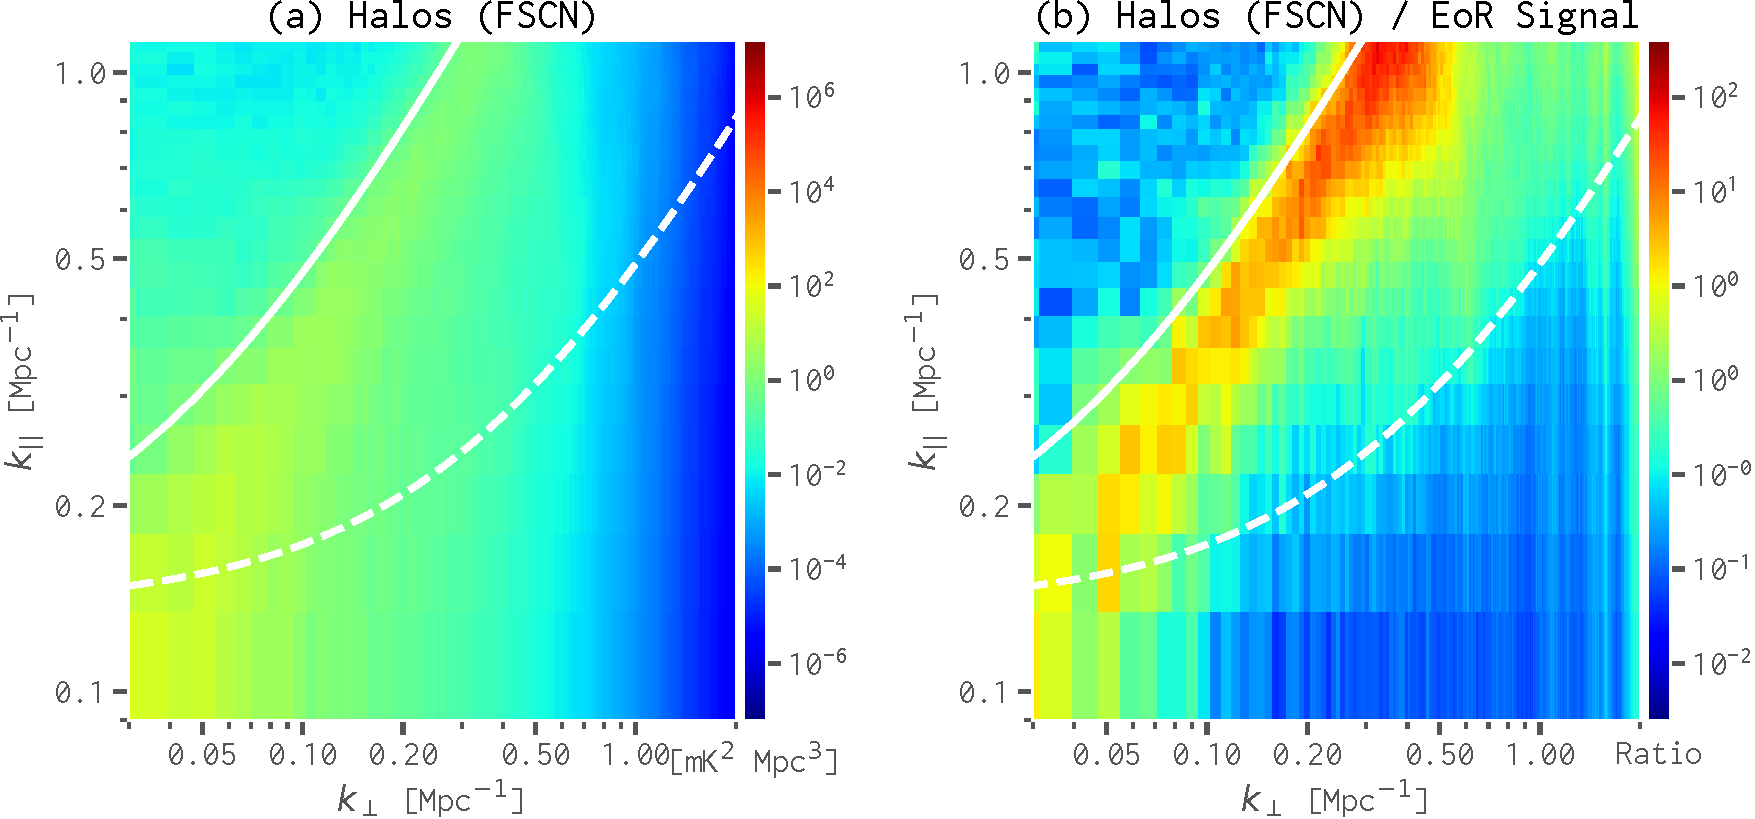
\includegraphics[width=\textwidth]{ps2d-fscn}
  \bicaption[远旁瓣里的射电晕的二维功率谱及其与 EoR 信号的功率谱对比]{%
    TODO...
  }{%
    \textbf{(a)} The 2D power spectrum of the FSCN caused by radio halos
    in the far side-lobes of the station beam.
    \textbf{(b)} The 2D power spectrum ratio of the FSCN to the EoR signal.
    The results are derived in the \SIrange{154}{162}{\MHz} band.
    The dashed and solid white lines mark the EoR window boundaries
    defined with $\Theta = \SI{6}{\degree}$ and \SI{90}{\degree},
    respectively.
  }
  \label{fig:ps2d-fscn}
\end{figure}

In \autoref{fig:ps2d-fscn}, we present the 2D power spectrum of the FSCN
contributed by radio halos and the corresponding 2D power spectrum ratio
of the FSCN to the EoR signal.
We find that the FSCN contamination is very strong as its power can be
about 20 times the power of the EoR signal on scales of
$\kperp \sim \SI{0.3}{\per\Mpc}$ and $\klos \sim \SI{1.0}{\per\Mpc}$.
The wedge-shaped contamination region moves toward the top left in
the $(\kperp, \klos)$ plane and greatly reduces the EoR window.
In order to effectively avoid the FSCN contamination, we are forced to
employ a much more conservative EoR window boundary, such as the one
defined with $\Theta = \SI{90}{\degree}$ as marked in
\autoref{fig:ps2d-fscn} with solid white line, at the cost of losing
a remarkably larger portion of the EoR signal.
In consequence,
the serious FSCN contamination makes the selection of EoR sky region
a more challenging task, since in principle neither bright radio halos
nor other strong sources are allowed in both the main and side lobes.
A highly accurate foreground model is hence crucial to mitigate the
impacts of FSCN.


%=====================================================================
\section{小结}

Based on the Press--Schechter formalism and merger-induced turbulent
re-acceleration model, we have simulated the emission maps of radio halos,
for which we have incorporated the SKA1-Low's instrumental effects by
utilizing its latest layout configuration.
By carrying out detailed comparisons of power spectra between radio halos
and the EoR signal as well as the Galactic diffuse emission and
extragalactic point sources in the \numrange{120}{128},
\numrange{154}{162}, and \numrange{192}{200} \si{\MHz} bands,
we have shown that radio halos are severe contaminating sources,
especially toward lower frequencies (\SI{\sim 120}{\MHz}).
Even if inside the properly defined EoR windows, radio halos can still
be non-negligible contaminating sources to EoR observations.
Moreover, we have investigated the contamination resulted from
frequency artifacts and radio halos located inside the far side-lobes,
both of which support our conclusion that radio halos are severe
foreground contaminating sources and need careful treatments in the
forthcoming deep EoR observations.

此工作已发表于 \apj{} (ApJ)\reviewornot{}{\cite{li.halo}}.


%% EOF
